\documentclass[paper=a4, fontsize=11pt]{scrartcl} % A4 paper and 11pt font size

\usepackage[T1]{fontenc}
\usepackage[utf8]{inputenc}
\usepackage[spanish, es-tabla]{babel}

%paquetes matematicos que igual necesitamos
\usepackage{amsmath,amsfonts,amsthm}
\usepackage{graphics,graphicx, float, url}
\newtheorem{teo}{Teorema}[section]
\setlength\parindent{0pt}

\numberwithin{equation}{section}
\newcommand{\horrule}[1]{\rule{\linewidth}{#1}} % Create horizontal rule command with 1 argument of height


\title{	
\normalfont \normalsize 
\textsc{{\bf Métodos Numéricos (2015-2016)} \\ Grado en Ingeniería Informática y Matemáticas \\ Universidad de Granada} \\ [25pt] % Your university, school and/or department name(s)
\horrule{0.5pt} \\[0.4cm] % Thin top horizontal rule
\huge Métodos de Runge-Kutta % The assignment title
\horrule{1pt} \\[0.5cm] % Thick bottom horizontal rule
}

\author{Pilar Espinosa de los Monteros Manero \\ Marina Estévez Almenzar \\ Elena Toro Pérez }
\date{April 2016}

\begin{document}
\maketitle

\newpage %inserta un salto de página

\tableofcontents % para generar el índice de contenidos
\pagebreak

	\section{Introducción}
	 Una de las herramientas matemáticas más efectivas de las que disponemos actualmente para modelizar y explicar la naturaleza son las \textbf{ecuaciones diferenciales}. Muchos problemas de las Ciencias y las Ingenierías se plantean mediante la resolución de un textbf{problema de valores iniciales}, en el que las ecuaciones diferenciales juegan un papel importante. Sin embargo, una resolución exacta de dicho problema no siempre es posible, principalmente por la imposibilidad o complejidad de resolver de forma explícita las ecuaciones diferenciales involucradas en el problema.
	\newline
	Se quiere hallar la solución de $y(x)$, que suponemos que existe y que es única en el intervalo $[a,b]$, de un problema de valores iniciales
	\newline
	\begin{equation*}
		(*)  \begin{cases} 
		&\text{$y'(x) = f(x,y)$}
		\\
		&\text{$y(x_0) = c$} 
		\end{cases} 
	\end{equation*}
	donde $y'(x) = f(x,y)$ puede ser una ecuación diferencial de orden 1, o un sistema de ecuaciones diferenciales de orden 1. Nos centraremos en la resolución del problema supuesto el primer caso (una ecuación diferencial de orden 1).
	El problema, por tanto, consiste en encontrar la función $y(x)$ que es solución única del problema.
	\newline\newline
	\textbf{¿Cómo?}
	\newline
	 Se usan métodos que tratan de aproximar la única solución $y(x)$ de dicho problema, entre ellos, los más usados y los que abarcan los métodos de \textit{Runge-Kutta} son los \textbf{métodos de discretización}.
	 \newline\newline
	 \textbf{Métodos de discretización}
	 \newline
	 Sea $(*)$ nuestro problema de valores iniciales. Supongamos que la función $f$ de nuestro problema está definida en $[a,b]\times\mathbb{R}$. Un método de discretización para resolverlo es cualquier método numérico que trata de obtener valores aproximados $y_n$ de la solución de $y(x)$ en los distintos nodos $x_n$ con $n={0,1,...,N}$ obtenidos mediante la partición del intervalo $[a,b]$.
	 \newline\newline
	 Estos métodos de discretización, además de abarcar los métodos de \textit{Runge-Kutta} que se exponen a continuación, también abarcan otros métodos como el método de \textit{Euler} o los métodos de \textit{Taylor}.
	 \newline
	 Veamos una definición esquematizada del método de \textit{Runge-Kutta} de $M$ evaluaciones (que posteriormente desarrollaremos para distintos valores de $M$):
	 \newline
	 Dado el problema de valores iniciales $(*)$ se define
	 \begin{equation*}
	 (1)\begin{cases} 
	 &\text{$y_0 = y(x_0)$}
	 \\
	 &\text{$y_{k+1} = y_k + h\phi(x_k,y_k,h) , k= 0,1,...,N-1$} 
	 \end{cases} 
	 \end{equation*}
	 donde
	 \begin{itemize}
	 	\item $h=\frac{a}{N} , N\in\mathbb{N}$
	 	\item $x_k = x_0 + kh , k=0,...,N$
	 	\item $\phi(x,y,h) = \sum_{j=1}^{M}c_jK_j(x,y,h)$ con $K_i(x,y,h)=f(x+ha_i,y+h\sum_{j=1}^{M}b_{ij}K_j(x,y,h))$ para $i=1,...,M$ y $c_i, a_i, b_{ij}$ constantes
	 \end{itemize}
	 Los métodos de \textit{Runge-Kutta} de $M$ evaluaciones que veremos se suelen representar mediante una tabla que contiene los coeficientes que determinan el método: \newline\textbf{la tabla de Butcher}
	 
	 \begin{table}[h]
	 	\begin{equation*}
	 	% \label{eq:19}
	 	\begin{array}{l | c c c c c}
	 	\rule{0pt}{2,3ex} a_1    \quad & \quad b_{11}  & \quad \cdots   &              & \quad b_{1M} &   \\
	 	\rule{0pt}{2,3ex} a_2    \quad & \quad b_{21}  &              &              & \quad b_{2M}        &   \\
	 	\rule{0pt}{2,3ex} \vdots \quad & \quad \vdots & \quad \vdots & \quad \ddots &         &   \\
	 	\rule{0pt}{2,3ex} a_M    \quad & \quad b_{M1}  & \quad \cdots  & \quad \cdots & \quad b_{MM} & \\[2,0ex] \hline
	 	\rule{0pt}{3,3ex}              & \quad c_{1}  & \quad c_{2}    & \quad \cdots & \quad c_{M}  & 
	 	\end{array}
	 	\end{equation*}
	 \end{table}
	 
 	 \textbf{Algunas definiciones previas necesarias para el estudio de los métodos}\newline
 	 \newline\textbf{Definiciones: error de truncamiento local y global}\newline
 	 Se define
 	 \newline $u_{k+1}=y(x_{k+1})-y(x_k)-h\phi(x_k,y(x_k),h)$ con $k=0,1,...,N-1$ como los \textit{errores de truncamiento/discretización locales} del método. 
 	 \newline A $e_k=y(x_k)-y_k$ se le llama \textit{error de truncamiento/discretización global}, siendo $x_k$ los nodos de la partición del intervalo, $y_k$ los valores aproximados de la solución $y(x)$ en el nodo $x_k$, con $k=0,...,N$.
 	 \newline
 	 Para estudiar la convergencia de estos métodos es necesario introducir los conceptos de \textbf{estabilidad} y \textbf{consistencia}:\newline
 	 \newline\textbf{Definición}\newline
 	 Un método de la forma (1)
 	 se dice \textbf{estable} si existen $M_1$ y $M_2$ tales que para cualquier par de conjuntos ${y_k}$ y ${z_k}$ definidos por
 	 \begin{equation*}
 	 \begin{cases} 
 	 &\text{$y_{k+1} = y_k+h\phi(x_k,y_k,h)$   con $y_0$ dado}
 	 \\
 	 &\text{$z_{k+1} = z_k+h\phi(x_k,z_k,h)+\varepsilon_k$    con $z_0$ dado} 
 	 \end{cases} 
 	 \end{equation*}
 	 se tiene que\newline
 	 $\max|y_k-z_k|\leq M_1|y_0-z_0|+M_2\max|\varepsilon_k|$\newline
 	 \newline Es importante hacer algunas observaciones de interés:
 	 \begin{itemize}
 	 	\item Las constantes $M_1$ y $M_2$ no dependen de $h$ y por tanto la estabilidad no depende del p.v.i. planteado.
 	 	\item La característica de estabilidad en un método indica que pequeñas perturbaciones en los datos de entrada originan pequeñas perturbaciones en los valores que se van obteniendo en el método.
 	 \end{itemize}
 	 \textbf{Definición}\newline
 	 Un método de la forma (1)
 	 se dice \textbf{consistente} con el p.v.i. $(*)$ cuando se verifica que
 	 \newline
 	 $\lim_{h \rightarrow 0}(\max \frac{|u_{k+1}|}{h}) = 0$
 	 \newline
 	 siendo $u_{k+1}=y(x_{k+1}-y(x_k)-h\phi(x_k,y(x_k),h)$ el error de truncamiento local, con  $k=0,1,...,N-1$.\newline
 	 \newline
 	 Un resultado importante que relaciona \textbf{estabilidad} y \textbf{consistencia} es el siguiente:
 	 
 	 \begin{center}
 	 	\fbox{
 	 		\begin{minipage}{1.0\textwidth}
 	 			Si un método de la forma $(1)$ es estable y consistente con un p.v.i. de la forma $(*)$ entonces dicho método converge a la solución de $(*)$
 	 		\end{minipage}
 	 	}
 	 \end{center}
 	 \textbf{Algunas observaciones sobre los métodos de Runge-Kutta que vamos a estudiar}
 	 \begin{itemize}
 	 	\item Un método de Runge-Kutta se dice que es \textit{explícito} cuando $b_{ij}=0$ para $j\geq i$
 	 	\item Si $f$ y $\phi$ son continuas, entonces\newline el método de Runge-Kutta es \textit{consistente} $\iff$ $\sum_{j=1}^{M}c_j=1$
 	 	\item Para simplificar los métodos de Runge-Kutta se exige que $a_i=\sum_{j=1}^{M}b_{ij}$
 	 \end{itemize}
	\section{Métodos de Runge-Kutta}
	\subsection{Método del punto medio}
	Sea f una función definida en $[x\textsubscript{0},x\textsubscript{0}+a] x \mathbb{R}$.
	Sea la ecuación diferencial de orden 1
	\begin{equation*}
	\left\lbrace
	\begin{array}{l}
	\ y^\prime = f(x,y) \\
	\ y(x\textsubscript{0}) = \eta \\
	\end{array}
	\right.
	\end{equation*}
	un p.v.i de ecuación $y^\prime = f(x,y)$ y condición inicial $y(x\textsubscript{0}) = \eta$ con solución única $y(x)$ en $[x\textsubscript{0},x\textsubscript{0}+a]$.
	
	\setlength{\parskip}{10pt}El método del \textbf{punto medio o Euler Modificado} es el método de Runge-Kutta en el que se utiliza el valor de la función f(x,y) evaluado en el punto medio entre $x\textsubscript{k}$ y $x\textsubscript{k}+h$, tomando en ese punto $x\textsubscript{k} + \frac{h}{2}$, el valor obtenido mediante el método de Euler.
	
	\subsubsection{Descripción}
	El método del punto medio es el método de Runge-Kutta de 2 evaluaciones cuyo tablero de Butcher es
	\begin{center}
		$\begin{array}{c|ccc}
		{a\textsubscript{1} = 0}\\
		{a\textsubscript{2} = 1/2}&{b\textsubscript{21} = 1/2}\\
		\hline
		{}&{c\textsubscript{1} = 0}&{c\textsubscript{2} = 1}\\
		\end{array}$
	\end{center}
	es decir:
	\begin{center}
		$\begin{array}{c|ccc}
		{0}\\
		{1/2}&{1/2}\\
		\hline
		{}&{0}&{1}\\
		\end{array}$
	\end{center}
	tal que:
	\begin{center}
		
		$\Phi(x,y,h) = K\textsubscript{2}(x,y,h)$
		
	\end{center}
	
	siendo:\\
	\begin{center}
		
		$K\textsubscript{1}(x,y,h) = f(x,y)$\\
		
		\setlength{\parskip}{10pt}$K\textsubscript{2}(x,y,h) = f(x + \frac{h}{2},y + \frac{h}{2}K\textsubscript{1}(x,y,h))$
		
	\end{center}
	Más concretamente, el método del punto medio para resolver dicha ecuación diferencial de orden 1, consiste en hallar $y\textsubscript{k} \in \mathbb{R}$ para $k = 0,1,...,N$, siendo $N \in \mathbb{N}-\lbrace0\rbrace$, mediante el siguiente proceso:
	
	\begin{center}
		\textbf{1º)} $y\textsubscript{0} = y(x\textsubscript{0})$
		
		\setlength{\parskip}{10pt}\textbf{2º)} $y\textsubscript{k+1} = y\textsubscript{k} + hf(x\textsubscript{k} + \frac{h}{2}, y\textsubscript{k} + \frac{h}{2}f(x\textsubscript{k}, y\textsubscript{k}))$, con $k = 0, ..., N-1$
	\end{center}
	
	donde $h = \frac{a}{N}$ y $x\textsubscript{k} = x\textsubscript{0} + kh$, con $k = 0,...,N$.\\
	
	A la segunda igualdad anterior se le llama \textbf{ecuación en diferencias del método del punto medio}.\\
	
	
	\subsubsection{Observación: Deducción del método del Punto Medio a partir de integración numérica}
	La ecuación en diferencias del método del punto medio para resolver la ecuación diferencial de orden 1 de la que estamos hablando, puede obtenerse igualando, para cada $k = 0,...,N-1$, las expresiones que resultan de sustituir $y(x\textsubscript{k+1})$ e $y(x\textsubscript{k})$ por $y\textsubscript{k+1}$ e $y\textsubscript{k}$, respectivamente, en los dos miembros de la aproximación\\
	\begin{center}
		$y(x\textsubscript{k+1}) \simeq y(x\textsubscript{k}) + hf(x\textsubscript{k} + \frac{h}{2}, y\textsubscript{k} + \frac{h}{2}f(x\textsubscript{k},y\textsubscript{k}))$
	\end{center}
	
	\setlength{\parskip}{10pt}que se deduce de la igualdad
	\begin{center}
		$y(x\textsubscript{k+1})- y(x\textsubscript{k}) = \int_{x\textsubscript{k}}^{x\textsubscript{k+1}} y\prime(x) dx = \int_{x\textsubscript{k}}^{x\textsubscript{k+1}} f(x, y(x)) dx$
	\end{center}
	
	usando la fórmula del punto medio para aproximar dicha integral, y aproximando el valor $y(x\textsubscript{k} + \frac{h}{2})$ que aparece en dicha fórmula usando el método de Euler de tamaño de paso $\frac{h}{2}$.
	
	
	Es decir, usando la integración numérica:
	\begin{center}	
		$\int_{x\textsubscript{k}}^{x\textsubscript{k+1}} y\prime(x) dx = \int_{x\textsubscript{k}}^{x\textsubscript{k+1}} f(x, y(x)) dx$
		
		\setlength{\parskip}{10pt}entonces:	
		
		\setlength{\parskip}{10pt}$y(x\textsubscript{k+1}) - y(x\textsubscript{k}) = \int_{x\textsubscript{k}}^{x\textsubscript{k+1}} f(x, y(x)) dx$
	\end{center}
	
	\setlength{\parskip}{10pt}con $k = 0, ..., N-1$.
	
	Supongamos $y\textsubscript{k}	\sim y(x\textsubscript{k})$, para $k \geq 1$ (e $y\textsubscript{0} = y(x\textsubscript{0})$ valor inicial).
	Sea el intervalo $[x\textsubscript{k}, x\textsubscript{k+1}]$, entonces el punto medio de dicho intervalo es $\frac{x\textsubscript{k} + x\textsubscript{k+1}}{2}$.
	
	Sea $h$ la longitud del intervalo $[x\textsubscript{k}, x\textsubscript{k+1}]$ y $\frac{h}{2}$ la longitud de sendos intervalos $[x\textsubscript{k}, \frac{x\textsubscript{k} + x\textsubscript{k+1}}{2}]$ y $[\frac{x\textsubscript{k} + x\textsubscript{k+1}}{2}, x\textsubscript{k+1}]$, podemos deducir:
	\begin{center}
		$\frac{x\textsubscript{k} + x\textsubscript{k+1}}{2} = x\textsubscript{k} + \frac{h}{2}$.
	\end{center}
	
	Por tanto, se obtiene:
	\begin{center}
		$y\textsubscript{k+1} - y\textsubscript{k} = (x\textsubscript{k+1} - x\textsubscript{k})f(x\textsubscript{k} + \frac{h}{2}, y\textsubscript{k} + \frac{h}{2}f(x\textsubscript{k}, y\textsubscript{k}))$
		
		de donde, finalmente:
		
		$y\textsubscript{k+1} = y\textsubscript{k} + hf(x\textsubscript{k} + \frac{h}{2}, y\textsubscript{k} + \frac{h}{2}f(x\textsubscript{k}, y\textsubscript{k}))$
	\end{center}
	
	
	\subsubsection{Estudio del error y análisis de la convergencia}
	Sea la forma general de los métodos de un paso generales
	\begin{center}
		$y\textsubscript{k+1} = y\textsubscript{k} + h\Phi(x\textsubscript{k},y\textsubscript{k},h)$
	\end{center}
	se define el \textbf{error local de discretización} en el punto x\textsubscript{k+1} como la cantidad:
	\begin{center}
		$\varepsilon\textsubscript{k+1}(h) = \frac{1}{h}(y(x\textsubscript{k+1}) - y(x\textsubscript{k}) - h\Phi(x\textsubscript{k},y(x\textsubscript{k}),h))$
	\end{center}
	y el \textbf{error global} como:
	\begin{center}
		$e\textsubscript{k+1} = y(x\textsubscript{k+1}) - y\textsubscript{k+1}$
	\end{center}
	
	Por construcción, el método del punto medio tiene la misma razón de convergencia que el método de Taylor de orden 2, es decir, $O(h^2)$.
	
	Es decir, este método tiene un error local de $O(h^3)$, y global de $O(h^2)$.
	
	\begin{teo}
		Sea $f: [x\textsubscript{0}, x\textsubscript{0}+a] x \mathbb{R} \rightarrow \mathbb{R}$ contínua y \textit{Lipschitziana} en su segunda variable. Entonces, el método del punto medio para resolver el p.v.i. $(1)$ de ecuación $y^\prime = f(x,y)$ y condición inicial $y(x\textsubscript{0}) = \eta$:
			\begin{itemize}
				\item Es estable
				\item Es consistente con el p.v.i. $(*)$
				\item Converge a la solución de $(*)$
			\end{itemize}
			Además, el método del punto medio es de orden 2. Es decir, el número de veces que se evalúa la función en cada paso del método es 2.
		\end{teo}
	
	
	
	\subsubsection{Ventajas y Desventajas en comparación con los otros métodos}
	Dicho método, junto con los demás de Runge-Kutta, son más sencillos que los de Taylor y, además, su convergencia es rápida.
	
	Los métodos de Taylor proporcionan una convergencia rápida, pero su implementación es complicada, ya que es necesario calcular los valores aproximados de las derivadas sucesivas de la solución. En contraposición, con los métodos de Runge-Kutta no necesitamos evaluar las derivadas sucesivas y, sin embargo, obtenemos convergencia rápida.
	
	El método de Euler, en cambio, es muy sencillo de aplicar, pero sin embargo su convergencia es lenta. En contraposición, los métodos de Runge-Kutta son también fáciles de aplicar, pero con ellos obtenemos una convergencia rápida.
	
	En el punto medio, el error global que se comete es de orden 2, con lo cual aunque la fórmula sea tan sencilla como la de Euler, la convergencia es mejor.
	
	Dicho método, en comparación con los demás métodos de Runge-Kutta, podemos deducir que se usa en menos casos que, por ejemplo, Runge-Kutta de orden 4 ya que este último nos proporciona mejor orden de convergencia y menor error global y en cada paso.
	
	\subsubsection{Ejemplo y ejercicio teórico/práctico}
	\textbf{Ejercicio 2: Sea \begin{equation*}
		\left\lbrace
		\begin{array}{l}
		\ y^\prime = 1 - x + 4y \\
		\ y(0) = 1 \\
		\end{array}
		\right.
		\end{equation*} queremos aproximar la solución en $x=1$ con distintos tamaños de paso: $h=0.1$ y $h=0.05$}.
	
	Como comenzamos con $x\textsubscript{0} = 0$ y queremos llegar hasta $x = 1$, serán necesarias $\frac{|x - x\textsubscript{0}|}{h = 0.1} = 10$ iteraciones en este caso.
	
	Realizando las sucesivas iteraciones con $h = 0.1$ y el método del punto medio obtenemos:
	\begin{itemize}
		\item $x\textsubscript{0} = 0$ e $y\textsubscript{0} = 1$
		\item $x\textsubscript{1} = 0.1$ e $y\textsubscript{1} = 1.595$
		\item $x\textsubscript{2} = 0.2$ e $y\textsubscript{2} = 2.463600000000001$
		\item $x\textsubscript{3} = 0.3$ e $y\textsubscript{3} = 3.737128000000001$
		\item $x\textsubscript{4} = 0.4$ e $y\textsubscript{4} = 5.609949440000002$
		\item $x\textsubscript{5} = 0.5$ e $y\textsubscript{5} = 8.369725171200003$
		\item $x\textsubscript{6} = 0.6$ e $y\textsubscript{6} = 12.442193253376$
		\item $x\textsubscript{7} = 0.7$ e $y\textsubscript{7} = 18.45744601499649$
		\item $x\textsubscript{8} = 0.8$ e $y\textsubscript{8} = 27.3480201021948$
		\item $x\textsubscript{9} = 0.9$ e $y\textsubscript{9} = 40.4940697512483$
		\item $x\textsubscript{10} = 1$ e $y\textsubscript{10} = 59.93822323184749$
	\end{itemize}
	
	La solución exacta es $64,897803$. Por tanto, el \textbf{error global} obtenido con $h = 0.1$ es: $4.95958$.
	
	
	Para $h = 0.05$, serán necesarias $\frac{|x - x\textsubscript{0}|}{h = 0.05} = 20$ iteraciones en este caso.
	
	Realizando las sucesivas iteraciones con $h = 0.05$ y el método del punto medio obtenemos:
	\begin{itemize}
		\item $x\textsubscript{0} = 0$ e $y\textsubscript{0} = 1$
		\item $x\textsubscript{1} = 0.05$ e $y\textsubscript{1} = 1.27375$
		\item $x\textsubscript{2} = 0.1$ e $y\textsubscript{2} = 1.604975$
		\item $x\textsubscript{3} = 0.15$ e $y\textsubscript{3} = 2.0063195$
		\item $x\textsubscript{4} = 0.2$ e $y\textsubscript{4} = 2.49320979$
		\item $x\textsubscript{5} = 0.25$ e $y\textsubscript{5} = 3.0844659438$
		\item $x\textsubscript{6} = 0.3$ e $y\textsubscript{6} = 3.803048451436$
		\item $x\textsubscript{7} = 0.35$ e $y\textsubscript{7} = 4.676969110751919$
		\item $x\textsubscript{8} = 0.4$ e $y\textsubscript{8} = 5.740402315117342$
		\item $x\textsubscript{9} = 0.45$ e $y\textsubscript{9} = 7.035040824443157$
		\item $x\textsubscript{10} = 0.5$ e $y\textsubscript{10} = 8.611749805820651$
		\item $x\textsubscript{11} = 0.55$ e $y\textsubscript{11} = 10.5325847631012$
		\item $x\textsubscript{12} = 0.6$ e $y\textsubscript{12} = 12.87325341098346$
		\item $x\textsubscript{13} = 0.65$ e $y\textsubscript{13} = 15.72611916139982$
		\item $x\textsubscript{14} = 0.7$ e $y\textsubscript{14} = 19.20386537690778$
		\item $x\textsubscript{15} = 0.75$ e $y\textsubscript{15} = 23.44396575982749$
		\item $x\textsubscript{16} = 0.8$ e $y\textsubscript{16} = 28.61413822698954$
		\item $x\textsubscript{17} = 0.85$ e $y\textsubscript{17} = 34.91899863692724$
		\item $x\textsubscript{18} = 0.9$ e $y\textsubscript{18} = 42.60817833705123$
		\item $x\textsubscript{19} = 0.95$ e $y\textsubscript{19} = 51.9862275712025$
		\item $x\textsubscript{20} = 1$ e $y\textsubscript{20} = 63.42469763686705$
	\end{itemize}
	
	La solución exacta es $64,897803$. Por tanto, el \textbf{error global} obtenido con $h = 0.05$ es: $1,473105$.
	
	\newpage
	\subsubsection{Método programado en Maxima}
	\textbf{PRIMERA IMPLEMENTACIÓN DEL MÉTODO}
	\begin{figure}[H]
		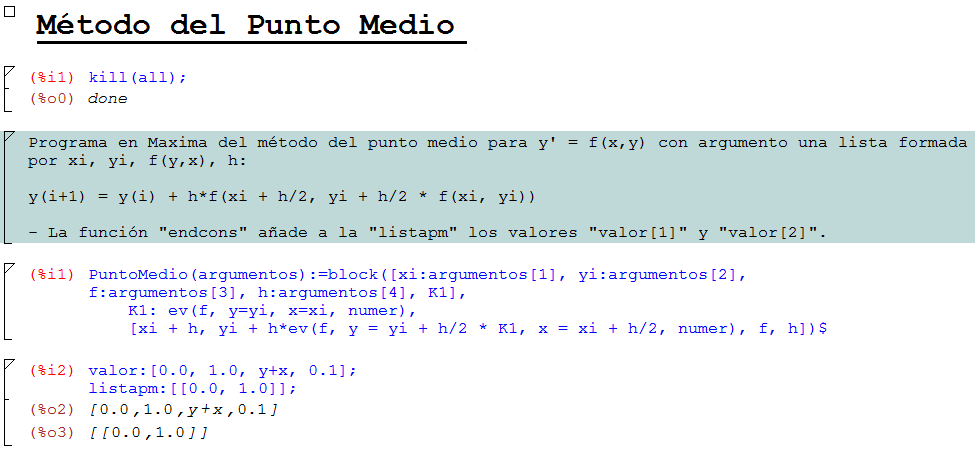
\includegraphics[width=1\textwidth]{Pm1.png}
		\caption{Punto Medio}
		\label{fig:Pm1}
	\end{figure}
	\begin{figure}[H]
		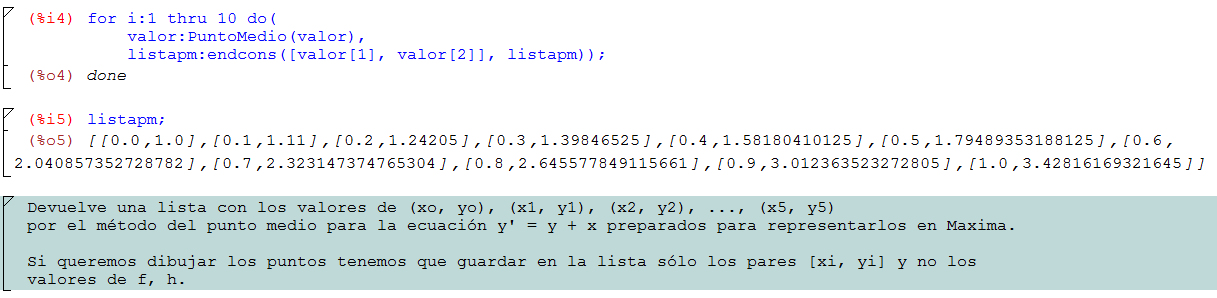
\includegraphics[width=1\textwidth]{Pm2.png}
		\caption{Punto Medio}
		\label{fig:Pm2}
	\end{figure}
	\begin{figure}[H]
		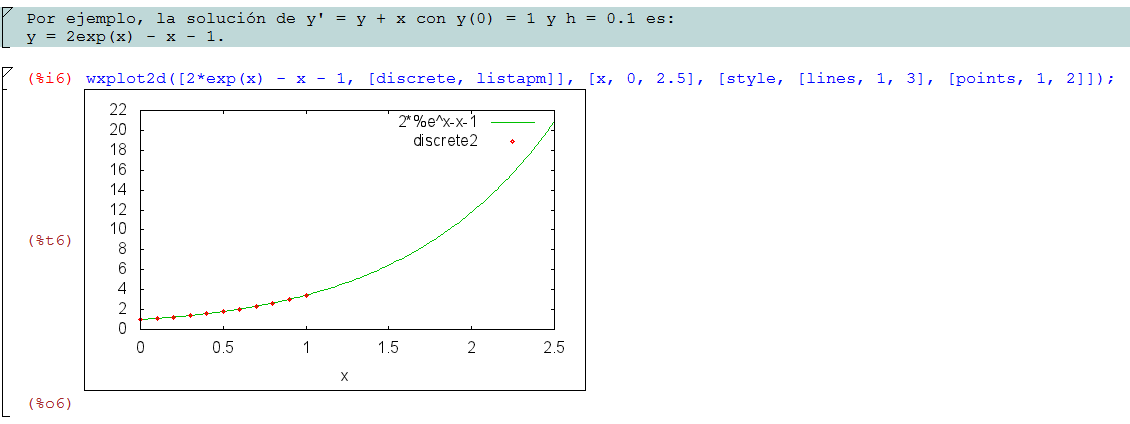
\includegraphics[width=1\textwidth]{Pm3.png}
		\caption{Punto Medio}
		\label{fig:Pm3}
	\end{figure}
	
	
	\textbf{SEGUNDA IMPLEMENTACIÓN DEL MÉTODO}
	\begin{figure}[H]
		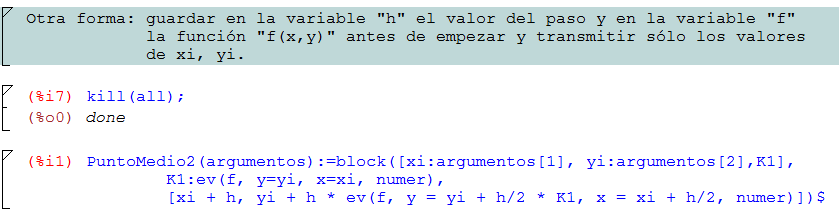
\includegraphics[width=1\textwidth]{Pm4.png}
		\caption{Punto Medio}
		\label{fig:Pm4}
	\end{figure}
	\begin{figure}[H]
		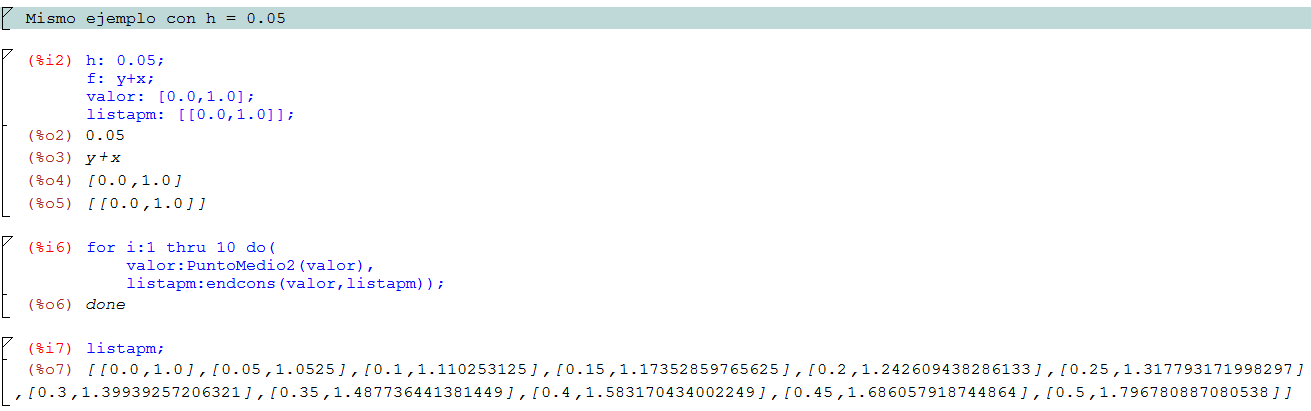
\includegraphics[width=1\textwidth]{Pm5.png}
		\caption{Punto Medio}
		\label{fig:Pm5}
	\end{figure}
	\begin{figure}[H]
		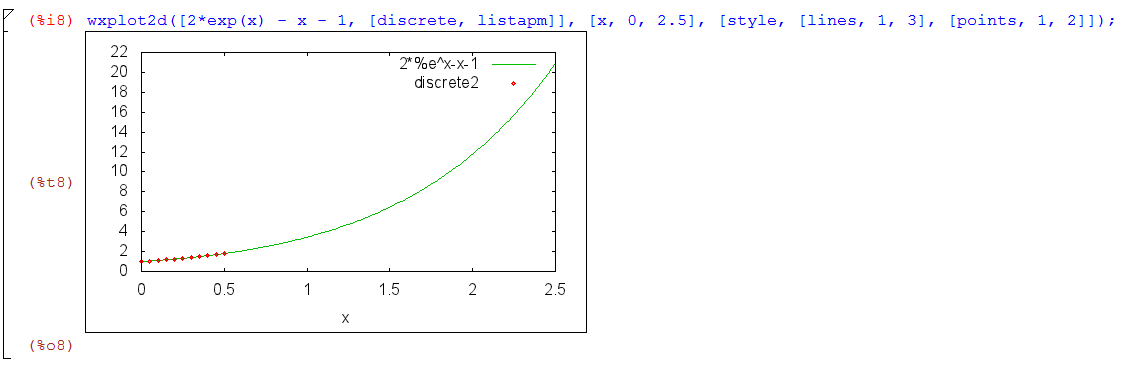
\includegraphics[width=1\textwidth]{Pm6.png}
		\caption{Punto Medio}
		\label{fig:Pm6}
	\end{figure}
	
	\textbf{TERCERA IMPLEMENTACIÓN DEL MÉTODO}
	\begin{figure}[H]
		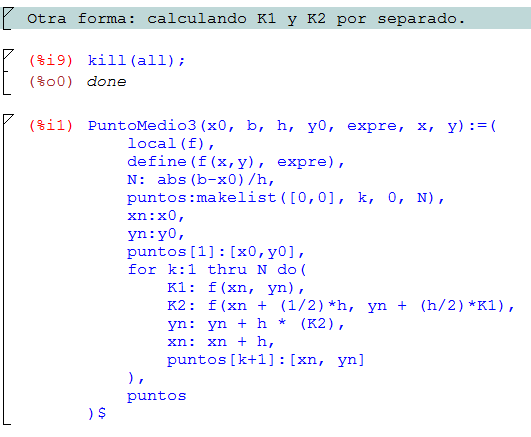
\includegraphics[width=1\textwidth]{Pm7.png}
		\caption{Punto Medio}
		\label{fig:Pm7}
	\end{figure}
	\begin{figure}[H]
		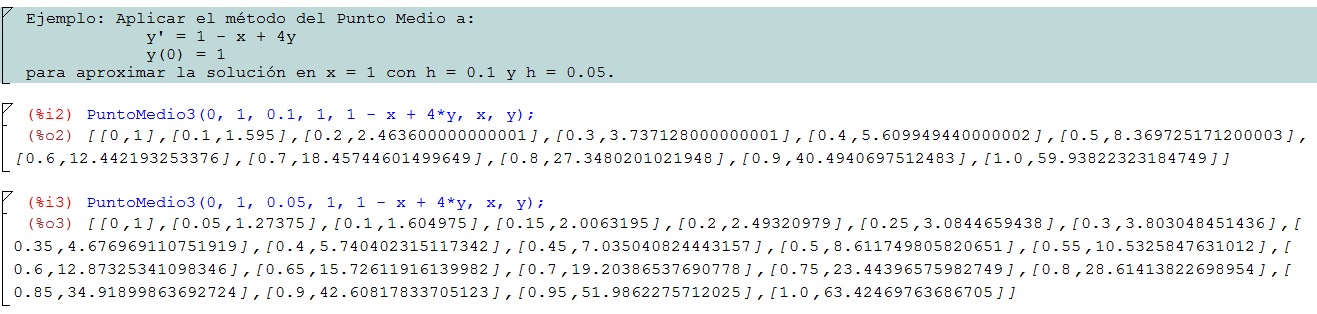
\includegraphics[width=1\textwidth]{Pm8.png}
		\caption{Punto Medio}
		\label{fig:Pm8}
	\end{figure}
	\begin{figure}[H]
		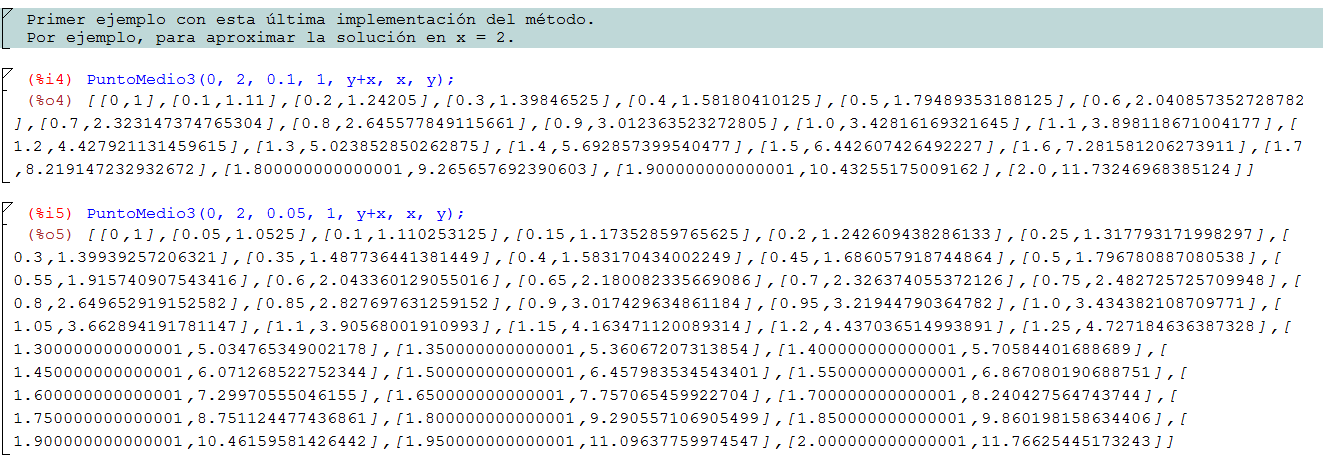
\includegraphics[width=1\textwidth]{Pm9.png}
		\caption{Punto Medio}
		\label{fig:Pm9}
	\end{figure}
	
	\subsection{Método de Runge-Kutta de orden 2}
	El método de \textbf{Runge-Kutta de orden 2} es una categoría que abarca diferentes métodos todos ellos haciendo uso de dos evaluaciones.
	\subsubsection{Método de Euler modificado}
	  Intenta refinar la aproximación a la pendiente de la función mediante la aplicación de dos derivadas en el intervalo, una en el punto inicial y otra en punto final. La aproximación mejorada de la pendiente será el promedio de las dos derivadas.\\
	Presenta la siguiente \textbf{tabla de Butcher}\begin{table}[h]
		\begin{equation*}
		% \label{eq:19}
		\begin{array}{l | c c c}
		\rule{0pt}{2,3ex} 0    \quad &   &  \\
		\rule{0pt}{2,3ex} 1 & 1 &  & \\[2,0ex] \hline
		\rule{0pt}{3,3ex}              & \quad 1/2  & 1/2  & 
		\end{array}
		\end{equation*}
	\end{table}
	\newpage
	Definimos el método como sigue:
	\begin{equation*}
	[RK2]\begin{cases} 
	&\text{$y_0 = y(x_0)$}
	\\
	&\text{$y_{k+1} = y_k + \frac{h}{2}(f(x_k,y_k)+f(x_k+h,y_k+hf(x_k,y_k))),  k= 0,1,...,N-1$} 
	\end{cases} 
	\end{equation*}
	
	donde:
	\begin{itemize}
		\item $h=\frac{a}{N} , N\in\mathbb{N}$
		\item $x_k = x_0 + kh , k=0,...,N$
		\item $\phi(x,y,h) = \frac{1}{2}(K_1+K_2)(x,y,h)$ con 
		\begin{itemize}
			\item $K_1(x,y,h)=f(x,y)$
			\item $K_2(x,y,h)=f(x+h,y+hK_1(x,y,h))$
		\end{itemize}
	\end{itemize}
	
	\subsubsection{Método de Heun}
	Este es también un método de segundo orden, que en las condiciones anteriores, tiene la forma:
	\begin{equation*}
	[RK2.2]\begin{cases} 
	&\text{$y_0 = y(x_0)$}
	\\
	&\text{$y_{k+1} = y_k + \frac{h}{4}(f(x_k,y_k)+3f(x_k+\frac{2}{3}h,y_k+\frac{2}{3}hf(x_k,y_k))),  k= 0,1,...,N-1$} 
	\end{cases} 
	\end{equation*}
	donde:
	\begin{itemize}
		\item $h=\frac{a}{N} , N\in\mathbb{N}$
		\item $x_k = x_0 + kh , k=0,...,N$
		\item $\phi(x,y,h) = \frac{1}{4}(K_1+3K_2)(x,y,h)$ con 
			\begin{itemize}
				\item $K_1(x,y,h)=f(x,y)$
				\item $K_2(x,y,h)=f(x+\frac{2}{3}h,y+\frac{2}{3}hK_1(x,y,h))$
			\end{itemize}
		\end{itemize}
	
	
	\subsubsection{Análisis de la convergencia y estudio del error}
	\textbf{Estudio de la convergencia}
	
	\begin{teo} Sea $f: [x\textsubscript{0}, x\textsubscript{0}+a]\times\mathbb{R} \rightarrow \mathbb{R}$ contínua, y lipschitziana en su segunda variable. Entonces el método de Runge-Kutta de orden 2 para resolver el p.v.i.$(*)$ de ecuación $y^\prime =f(x, y)$ y condición inicial $y(x_0) = \eta$ es
		\begin{itemize}
			\item Es estable
			\item Es consistente con $(*)$
			\item Converge a la solución de $(*)$
		\end{itemize}
		Además, el método $[RK2]$ es de orden 2.
	\end{teo}
	
	\textbf{Análisis del error}\\
	Sean $y_k$ el valor exacto de la función y $\overline{y_k}$ el valor aproximado conseguido con $k = 1,...,N$. Entonces:
	\begin{itemize}
		\item Se define el \textit{error de truncamiento del paso j} como $e_j =y_j-\overline{y_j}$
		\item Se define el \textit{error de truncamiento global} como $e_n =y_n-\overline{y_n}$
	\end{itemize}
	
	
	En cuanto al error podemos decir que por su definición el método RK2 tiene la misma razón de convergencia que el método de Taylor de orden 2, es decir, $O(h^2)$.
	
	Es decir, este método tiene un error local de $O(h^3)$, y global de $O(h^2)$.
	
	\textbf{Observaciones}
	De nuevo este método presenta una ventaja sobre los métodos de \textit{Taylor}, evitando el cálculo de las derivadas y la evaluación de las mismas. Es decir conlleva un cálculo computacionalmente menos pesado.\newline
	
	\subsubsection{Programación [RK2] y ejercicio numérico}
	Pseudocódigo para el método de Euler modificado.
	\begin{center}
		\fbox{
			\begin{minipage}{1.0\textwidth}
				$RK2(a,b,h,y(a),f)\newline
				N \leftarrow (b-a)/h\newline
				x_0 \leftarrow a\newline
				y_0 \leftarrow y(a)\newline
				for(i=0; i<N; i++)\{\newline
				\begin{tabular}{l}$
				K_1 \leftarrow f(x_i,y_i)\newline
				$\end{tabular}
				\newline
				\begin{tabular}{l}$
				p \leftarrow y_i + h*K_1 \newline
				$\end{tabular}
				\newline
				$\begin{tabular}{l}$
					x_{i+1} \leftarrow a+(i+1)*h
					$\end{tabular}
				\newline
				\begin{tabular}{l}$
					K_2 \leftarrow f(x_{i+1},p)\newline
					$\end{tabular}
				\newline
				\begin{tabular}{l}$
					y_{i+1}\leftarrow
					y_i+\frac{h}{2}(K_1+K_2)\newline
					$\end{tabular}$
				\newline \}$
			\end{minipage}
		}
	\end{center}
	
	Por lo tanto el código queda como sigue:
	
\begin{figure}[H]
	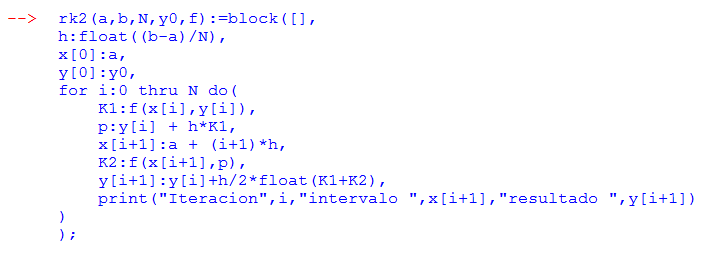
\includegraphics[width=1\textwidth]{rk2.png}
	\caption{Metodo de Euler modificado}
	\label{fig:Euler}
\end{figure}
	
	Pseudocódigo para el método de Heun
	\begin{center}
		\fbox{
			\begin{minipage}{1.0\textwidth}
				$RK2(a,b,h,y(a),f)\newline
				N \leftarrow (b-a)/h\newline
				x_0 \leftarrow a\newline
				y_0 \leftarrow y(a)\newline
				for(i=0; i<N; i++)\{\newline
				\begin{tabular}{l}$
				K_1 \leftarrow f(x_i,y_i)\newline
				$\end{tabular}
				\newline
				\begin{tabular}{l}$
				p \leftarrow y_i + \frac{2}{3}h*K_1 \newline
				$\end{tabular}
				\newline
				$\begin{tabular}{l}$
					x_{i+1} \leftarrow a+(i+1)*h
					$\end{tabular}
				\newline
				\begin{tabular}{l}$
					K_2 \leftarrow 3f(x_i+\frac{2}{3}h,p)\newline
					$\end{tabular}
				\newline
				\begin{tabular}{l}$
					y_{i+1}\leftarrow
					y_i+\frac{h}{4}(K_1+K_2)\newline
					$\end{tabular}$
				\newline \}$
			\end{minipage}
		}
	\end{center}
	
	\begin{figure}[H]
		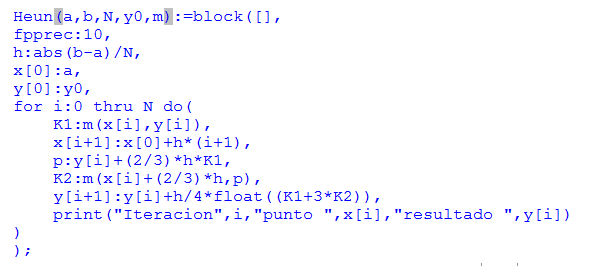
\includegraphics[width=1\textwidth]{heun.png}
		\caption{Metodo de Heun}
		\label{fig:Heun}
	\end{figure}
	
	
	\textbf{Ejemplo}: veamos un simple ejemplo que muestra la convergencia del método de Euler modificado.
	\begin{center}
		\fbox{
			\begin{minipage}{1.0\textwidth}
				Dado el siguiente p.v.i.:
				\begin{equation*}
				\begin{cases} 
				&\text{$y'(x) = f(x,y) = y + 2x - x^2$}
				\\
				&\text{$y(0) = -1$} 
				\end{cases} 
				\end{equation*}
				Aproximar el valor de $y(1)$ fijado un paso $h=0.2$
			\end{minipage}
		}
	\end{center}
	Ejecutando el método obtenemos los siguientes valores:\\
	\begin{tabular}[t]{|l |c | c |r|}
		\hline
		$x_n$ & $x_n$ & $y_n(x_n)$ & $|y_n - \overline{y_n}|$ \\
		\hline
		0 & -1.0000 & -1.000 & 0\\
		\hline
		0.2000 & -1.1840 & -1.1814 & 0.0026 \\
		\hline
		0.4000 & -1.3373 & -1.3318 & 0.0055\\
		\hline
		0.6000 & -1.4707 & -1.4621 & 0.0086\\
		\hline
		0.8000 & -1.5974 & -1.5855 & 0.0119\\
		\hline
		1.0000 & -1.7337 & -1.7183 & 0.0154\\
		\hline
	\end{tabular}\newline
	
	Otro ejemplo:
	\begin{center}
		\fbox{
			\begin{minipage}{1.0\textwidth}
				Dada el siguiente p.v.i.:
				\begin{equation*}
				\begin{cases} 
				&\text{$y'(x) = 2xy$}
				\\
				&\text{$y(1) = 1$} 
				\end{cases} 
				\end{equation*}
				Aproximar el valor de $y(1.5)$ fijado un paso $h=0.1$
			\end{minipage}
		}
	\end{center}
	
	\begin{figure}[H]
		\centering
		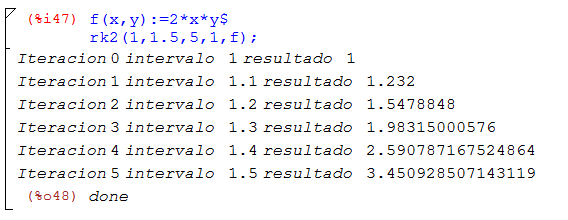
\includegraphics[width=10cm]{f1.png}
		\caption{Ejecución RK2}
		\label{fig:my_label}
	\end{figure}
	
	\subsection{Método de Runge-Kutta de orden 4}
	El \textbf{Método de Runge-Kutta de orden 4} (también llamado método de \textit{Runge-Kutta clásico} o \textit{Runge-Kutta de 4 evaluaciones}) viene dado por la siguiente \textbf{tabla de Butcher}\begin{table}[h]
		\begin{equation*}
		% \label{eq:19}
		\begin{array}{l | c c c c c}
		\rule{0pt}{2,3ex} 0    \quad &   &    &     &  &   \\
		\rule{0pt}{2,3ex} 1/2    \quad & \quad 1/2  &              &              &         &   \\
		\rule{0pt}{2,3ex} 1/2 & 0 & 1/2 &  &         &   \\
		\rule{0pt}{2,3ex} 1 & 0  & 0  & 1 &  & \\[2,0ex] \hline
		\rule{0pt}{3,3ex}              & \quad 1/6  & 2/6    & 2/6 & 1/6  & 
		\end{array}
		\end{equation*}
	\end{table}
	por tanto, el método se define como:
	\begin{equation*}
	[RK4]\begin{cases} 
	&\text{$y_0 = y(x_0)$}
	\\
	&\text{$y_{k+1} = y_k + \frac{h}{6}\phi(x_k,y_k,h) , k= 0,1,...,N-1$} 
	\end{cases} 
	\end{equation*}
	donde
	\begin{itemize}
		\item $h=\frac{a}{N} , N\in\mathbb{N}$
		\item $x_k = x_0 + kh , k=0,...,N$
		\item $\phi(x,y,h) = (K_1+2K_2+2K_3+K_4)(x,y,h)$ con 
		\begin{itemize}
			\item $K_1(x,y,h)=f(x,y)$
			\item $K_2(x,y,h)=f(x+\frac{h}{2},y+\frac{h}{2}K_1(x,y,h))$
			\item $K_3(x,y,h)=f(x+\frac{h}{2},y+\frac{h}{2}K_2(x,y,h))$
			\item $K_4(x,y,h)=f(x+h,y+hK_3(x,y,h))$
		\end{itemize}
	\end{itemize}
	\subsubsection{Análisis de convergencia y estudio del error}
	\textbf{Estudio de la convergencia}
	\newline
	En nuestro caso tenemos que, dado el método 
	\begin{equation*}
	[RK4]\begin{cases} 
	&\text{$y_0 = y(x_0)$}
	\\
	&\text{$y_{k+1} = y_k + \frac{h}{6}\phi(x_k,y_k,h) , k= 0,1,...,N-1$} 
	\end{cases} 
	\end{equation*}
	donde
	\begin{itemize}
		\item $h=\frac{a}{N} , N\in\mathbb{N}$
		\item $x_k = x_0 + kh , k=0,...,N$
		\item $\phi(x,y,h) = (K_1+2K_2+2K_3+K_4)(x,y,h)$ con 
		\begin{itemize}
			\item $K_1(x,y,h)=f(x,y)$
			\item $K_2(x,y,h)=f(x+\frac{h}{2},y+\frac{h}{2}K_1(x,y,h))$
			\item $K_3(x,y,h)=f(x+\frac{h}{2},y+\frac{h}{2}K_2(x,y,h))$
			\item $K_4(x,y,h)=f(x+h,y+hK_3(x,y,h))$
		\end{itemize}
	\end{itemize}
	\begin{center}
		\fbox{
			\begin{minipage}{1.0\textwidth}
				Si $f$ es \textit{Lipschitziana} en su segunda variable, entonces el método $[RK4]$ para resolver el p.v.i. $(*)$:
				\begin{itemize}
					\item Es estable
					\item Es consistente con $(*)$
					\item Converge a la solución de $(*)$
				\end{itemize}
				Además, el método $[RK4]$ es de orden 4.
			\end{minipage}
		}
	\end{center}
	\textbf{Estudio del error}
	\newline Se cumple que, dado el método 
	\begin{equation*}
	[RK4]\begin{cases} 
	&\text{$y_0 = y(x_0)$}
	\\
	&\text{$y_{k+1} = y_k + \frac{h}{6}\phi(x_k,y_k,h) , k= 0,1,...,N-1$} 
	\end{cases} 
	\end{equation*}
	donde
	\begin{itemize}
		\item $h=\frac{a}{N} , N\in\mathbb{N}$
		\item $x_k = x_0 + kh , k=0,...,N$
		\item $\phi(x,y,h) = (K_1+2K_2+2K_3+K_4)(x,y,h)$ con 
		\begin{itemize}
			\item $K_1(x,y,h)=f(x,y)$
			\item $K_2(x,y,h)=f(x+\frac{h}{2},y+\frac{h}{2}K_1(x,y,h))$
			\item $K_3(x,y,h)=f(x+\frac{h}{2},y+\frac{h}{2}K_2(x,y,h))$
			\item $K_4(x,y,h)=f(x+h,y+hK_3(x,y,h))$
		\end{itemize}
	\end{itemize}
	\begin{center}
		\fbox{
			\begin{minipage}{1.0\textwidth}
				Llamemos $\varepsilon_0$ al error de redondeo cometido en el dato inicial y, para $k=0,...,N$, llamemos $\varepsilon_k$ al error de redondeo cometido en el paso $k$, es decir:
				\begin{itemize}
					\item $z_0 = y_0 + \varepsilon_0$
					\item $z_{k+1}=z_k+\frac{h}{6}\phi(x_k,z_k,h)+\varepsilon_k$
				\end{itemize}
				Se cumple que si $\phi$ es \textit{Lipschitziana} en su segunda variable con constante de Lipschitz igual a $M$ se verifica que\newline
				\newline
				$\arrowvert E_k\arrowvert \leq e^{x_k-x_0}M \arrowvert\varepsilon_0\arrowvert+\frac{e^{(x_k-x_0)M}-1}{M}(\tau+\frac{\varepsilon}{h})$
				\newline
				\newline donde $E_k=z_k-y(x_k)$ , $\tau=\max_{k=0,1,...,N-1}\frac{\arrowvert u_{k+1}\arrowvert}{h}$ , $\varepsilon=\max_{k=0,1,...,N-1}\arrowvert\varepsilon_k\arrowvert$
			\end{minipage}
		}
	\end{center}
	
	\subsubsection{Ventajas y desventajas}
	\textbf{Ventajas}: \newline
	En comparación con los métodos de \textit{Taylor}, el método $[RK4]$ evita el cálculo de las derivadas, por lo que resulta computacionalmente menos pesado.\newline
	En comparación con los demás métodos de \textit{Runge-Kutta} se tiene que el error por paso es del orden de $O(h^5)$, mientras que el error acumulado es del orden de $O(h^4)$. Así, el orden de convergencia es de $O(h^4)$. Esta es la razón por la que $[RK4]$ es el método computacional más usado.
	
	\subsubsection{Ejercicio teórico-práctico}
	\begin{center}
		\fbox{
			\begin{minipage}{1.0\textwidth}
				Dada el siguiente p.v.i.:
				\begin{equation*}
				\begin{cases} 
				&\text{$x'(t) = -x+(t-1)y$}
				\\
				&\text{$y'(t) = x-ty$} 
				\end{cases} 
				\end{equation*}
				Con condiciones iniciales:
				\begin{equation*}
				\begin{cases} 
				&\text{$x(0)=0'483941$}
				\\
				&\text{$y(0)=0'682689$} 
				\end{cases} 
				\end{equation*}
				Utilizamos el método de Runge-Kutta se orden 4 para hallar los valores de $x(t)$ e $y(t)$ para $t=2\sqrt{2}-1 = 1'82843$
			\end{minipage}
		}
	\end{center}
	Por simplificar, vamos a calcular dicha aproximación en un solo paso, de forma que, como las condiciones iniciales son dadas para un tiempo $t_0=0$, el valor de $h$ debe ser $h=2\sqrt{2}-1 = 1'82843$. Nuestro método por tanto consiste en aplicar la siguiente iteración: \newline
	\newline
	${x_{i+1} \choose y_{i+1}} = {x_i \choose y_i} + \frac{h}{6}{r_1+2r_2+2r_3+r_4 \choose k_1+2k_2+2k_3+k_4}$\newline
	\newline 
	donde\newline
	\newline
	$r_1=f(t_y,x_i,y_i)\newline
	k_1=g(t_i,x_i,y_i)\newline
	r_2=f(t_i+\frac{h}{2},x_i+\frac{h}{2}r_1,y_i+\frac{h}{2}k_1)\newline
	k_2=g(t_i+\frac{h}{2},x_i+\frac{h}{2}r_1,y_i+\frac{h}{2}k_1)\newline
	r_3=f(t_i+\frac{h}{2},x_i+\frac{h}{2}r_2,y_i+\frac{h}{2}k_2)\newline
	k_3=g(t_i+\frac{h}{2},x_i+\frac{h}{2}r_2,y_i+\frac{h}{2}k_2)\newline
	r_4=f(t_i+h,x_i+hr_3,y_i+hk_3)\newline
	k_4=g(t_i+h,x_i+hr_3,y_i+hk_3)\newline$\newline
	\newline
	De esta forma, sustituyendo $h=2\sqrt{2}-1 = 1'82843$ nos queda que:\newline
	\newline
	$r_1=0'198748\newline
	k_1=0'483941\newline
	r_2=1'48807\newline
	k_2=-0'362958\newline
	r_3=-1'17272\newline
	k_3=1'52359\newline
	r_4=11'4706\newline
	k_4=-8'00215\newline$\newline
	\newline
	Y sustituyendo en la iteración dada por el método de Runge-Kutta se obtiene:\newline
	\newline
	$x(2\sqrt{2}-1) = x(1'82843) \approx x_1 = 4'23224\newline
	y(2\sqrt{2}-1) = y(1'82843) \approx y_1 = 0'90102\newline$
			
	\subsubsection{Programación de [RK4] y ejercicio numérico}
	Veamos a continuación el pseudocódigo del método:
	\begin{center}
		\fbox{
			\begin{minipage}{1.0\textwidth}
				$RK4(a,b,h,y(a),f)\newline
				N \leftarrow (b-a)/h\newline
				x_0 \leftarrow a\newline
				y_0 \leftarrow y(a)\newline
				for(i=0; i<N; i++)\{\newline
				$\begin{tabular}{l}$
					x_i \leftarrow a+i*h
				$\end{tabular}
				\newline
				\begin{tabular}{l}$
					K_1 \leftarrow h*f(x_i,y_i)\newline
				$\end{tabular}
				\newline
				\begin{tabular}{l}$
					K_2 \leftarrow h*f(x_i+\frac{1}{2}h,y_i+\frac{1}{2}K_1)\newline
				$\end{tabular}
				\newline
				\begin{tabular}{l}$
					K_3 \leftarrow h*f(x_i+\frac{1}{2}h,y_i+\frac{1}{2}K_2)\newline
				$\end{tabular}
				\newline
				\begin{tabular}{l}$
					K_4 \leftarrow h*f(x_i+h,y_i+K_3)\newline
				$\end{tabular}
				\newline
				\begin{tabular}{l}$
					y_{i+1}\leftarrow
					 y_i+\frac{1}{6}(K_1+2K_2+2K_3+K_4)\newline
				$\end{tabular}$
				\newline \}$
			\end{minipage}
		}
	\end{center}
	
	Visto esto, construimos el método en \textit{Maxima} para más tarde resolver un p.v.i. sencillo a modo de ejemplo. La construcción se encuentra en la Figura~\ref{fig:RK4}.
	\begin{figure}[H]
		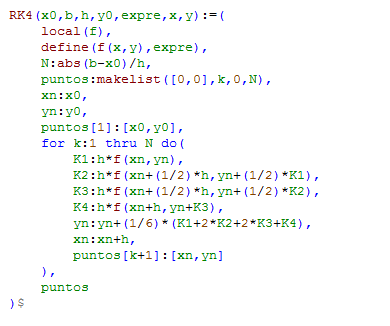
\includegraphics[width=0.75\textwidth]{rk.png}
		\caption{RK4}
		\label{fig:RK4}
	\end{figure}

	\newpage
	Resolvamos a continuación un sencillo p.v.i.:
	\begin{center}
		\fbox{
			\begin{minipage}{1.0\textwidth}
				Dada el siguiente p.v.i.:
				\begin{equation*}
					\begin{cases} 
					&\text{$y'(x) = 2xy$}
					\\
					&\text{$y(1) = 1$} 
					\end{cases} 
				\end{equation*}
				Aproximar el valor de $y(1.5)$ fijado un paso $h=0.1$
			\end{minipage}
		}
	\end{center}
	Tras la ejecución en \textit{Maxima} obtenemos:\newline
	$y(1)=1,0000$ (solución exacta: 1,0000)\newline
	$y(1.1)=1,2337$ (solución exacta: 1,2337)\newline
	$y(1.2)=1,5527$ (solución exacta: 1,5527)\newline
	$y(1.3)=1,9937$ (solución exacta: 1,9937)\newline
	$y(1.4)=2,6116$ (solución exacta: 2,6117)\newline
	$y(1.5)=3,4902$ (solución exacta: 3,4904)\newline
	\newline
	Con este mismo p.v.i. podemos ver una\textbf{ comparativa} de los tres métodos estudiados, expresada en la siguiente tabla:\newline
		\begin{tabular}[t]{|l |c|c |c |c |c |c | c | c |c|r|}
			\hline
			$Valor$ &$h$& $Pto$ $medio$ & $Euler2$ & $Heun$ & $RK4$ &$Err$ $MPM$&$Err$ $Euler$&$Err$$Heun$&$Err$$RK4$ \\
			\hline
			1,0000 &1,0& 1,0000 & 1.0000 &1,0000& 1,0000 & 0 & 0 &0& 0\\
			\hline
			1,2337&1,1& 1.231 & 1,232 & 1.2313 & 1,2337 & 0,0027 & 0.0017 &0.004& 0\\
			\hline
			1,5527&1,2& 1,5453 & 1,5479 &1.5461& 1,5527 & 0,0074 & 0.0048&0,0066& 0\\
			\hline
			1,9937&1,3& 1,9779 & 1,9832 & 1.9797& 1,9937 & 0.0158 & 0.0105& 0,014 &0\\
			\hline
			2,6117&1,4& 2,5814 & 2,5908 &2.5845& 2,6116 & 0,303 &  0,0209&0,0272& 0,0001\\
			\hline
			3,4904&1,5& 3,4348 & 3,4509 &3.4402& 3,4902 & 0,0556 & 0,0395& 0.0502&0.0002\\
			\hline
		\end{tabular}
\newpage
\subsection{Articulo}
El articulo \textit{"Zero-finder methods derived using Runge–Kutta techniques"} hace un estudio sobre la posibilidad de integrar los métodos de Runge-Kutta en un problema iterativo donde se busca el cero de la función. Runge-Kutta entra en juego cuándo se están tratando las derivadas de la función. Por lo tanto, se intenta simplificar el problema creando uno que ya conocemos como es el problema del valor inicial. La idea consiste en resolver una función diferencial que es a su vez inversa de una función  donde al computar el cero obtenemos el valor inicial. 

En consecuencia el problema toma la siguiente forma. Sea $f$ una función con raíz simple $\alpha$, $f(\alpha)=0$ teniendo que $f\prime(\alpha)\not=0$ en un entorno $I_\alpha$ de $\alpha$. Entonces existe la inversa de la función $x=g(y)$ en $J_0\subseteq f(I_\alpha)$ con $g(0)=\alpha$. Si derivamos la función $x(y)$ respecto de la $y$ se obtiene:

$\frac{dx}{dy} = g\prime(y) = \frac{1}{f\prime(x)}$

Puediendo expresarlo de la forma:
$x\prime(y) = F(x)$ siendo $F(x)=\frac{1}{f\prime(x)}$\\

Esto supone que, la ecuación $f(x)=0$ con una aproximación inicial $x_0$ puede resolverse como un problema de valor inicial con $x\prime(y) = F(x)$ siendo la condición inicial $y=y_0= f(x_0)$. El intervalo de trabajo tiene extremos $y_0$ y 0 ya que $g(y_0) = x_0$ y $g(0) = \alpha$.

En el estudio presentado se utilizan métodos de runge-Kutta de ordenes 1, 2 y 3 que combinándolo con el método iterativo de Newton mejoran el error cometido. Cabe destacar que a la hora de aplicar los diferentes métodos de Runge-Kutta se exige siempre que la raíz sea simple y que no se anule la derivada hasta un cierto grado, recordemos que tratamos con la inversa de una función diferencial, en ningún caso puede ser cero.\\

En resumen, el articulo propone una herramienta más para solucionar problemas que tratan con ecuaciones no lineales por medio de ecuaciones diferenciales. Confluyen así, en cierta medida, dos de los temas más importantes tratados en la asignatura. 

\newpage
\section{Referencias}

\begin{thebibliography}{10}
\expandafter\ifx\csname url\endcsname\relax
  \def\url#1{\texttt{#1}}\fi
\expandafter\ifx\csname urlprefix\endcsname\relax\def\urlprefix{URL }\fi
\expandafter\ifx\csname href\endcsname\relax
  \def\href#1#2{#2} \def\path#1{#1}\fi
\bibitem{1}
Análisis Matemático para Ingeniería. M. Molero; A. Salvador; T. Menarguez; L. Garmendia. Capitulo 13, pag. 36-53.\\
\url{http://www2.caminos.upm.es/Departamentos/matematicas/Fdistancia/PIE/Analisis%20matematico/Temas/C13_Metodo_Numerico.pdf}
\bibitem{2}
Apuntes del Tema 3 de la asignatura Métodos Numérico II de los profesores Teresa E. Pérez y Miguel Piñar. Curso 14/15.
\bibitem{3}
Apuntes del Tema 3 de la asignatura Métodos Numérico II de la profesora M. Carmen Serrano Pérez. Curso 13/14.
\bibitem{4}
Métodos numéricos con software libre: Maxima. María Santos Bruzón Gallego, José Ramírez Labrador. Capítulo 8, pág 156-159.
\bibitem{5}
Facultad Regional de San Nicolás: Métodos Numéricos para EDOs. Problemas de valor inicial y problemas de frontera.\\
\url{http://www.frsn.utn.edu.ar/gie/an/mnedo/34_RK.html}
\bibitem{6}
Métodos numéricos: problemas resueltos y prácticas. Isaac A. García, Susanna Maza.

\bibitem{7}
Bibligrafía recomendada en la hoja del trabajo.

\bibitem{8}
Zero-finder methods derived using Runge–Kutta techniques. Miquel Grau-Sánchez , José Luis Díaz-Barrero. Technical Universidad de Cataluña, Departmento de Matemáticas Aplicadas.\\
\url{http://www.sciencedirect.com/science/article/pii/S0096300310011926}

\end{thebibliography}
\end{document}